\makeheading{A Guide to Air Pollution and your Survival Index\\穹顶之下——空气污染、雾霾天生存防护指南}

\begin{multicols}{3}
\greyboxNID{\it
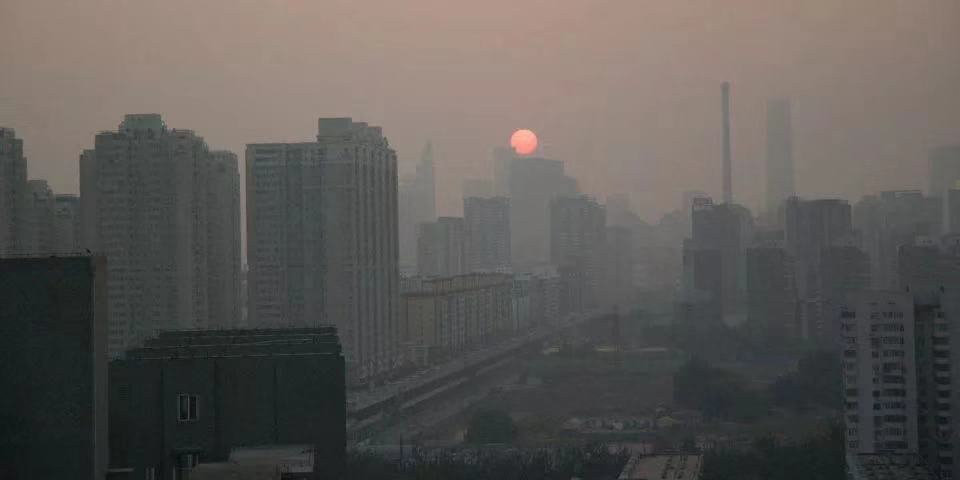
\includegraphics[width=\linewidth]{IMG/201912/image1.jpeg}

\quad\quad ``Wearing a mask is not good-looking at all, but if exposed to the turbid(浑浊的) air of Beijing, it will cause a sore throat in just 30 minutes."

\quad\quad “戴口罩一点儿都不好看,但暴露在北京浑浊的空气里,只要30分钟就会喉咙痛。”——《北京的蓝天》(Blue skies over Beijing)}


As the world gets hotter and more crowded, we continue to pump out dirty \textit{emissions(排放物)}, and half the world has no access to clean fuels or technologies , the very air we breathe is growing dangerously polluted: nine out of ten people now breathe polluted air, which kills 7 million people every year.

随着全球变暖和人口增长,我们持续排放大量污染物,且全球一半人口无法获得清洁的燃料或技术。我们呼吸的空气正危险地受到污染:世界上90\%的人口呼吸被污染的空气,每年造成700万人死亡。

To control the air pollution and reduce the negative health effects it \textit{imposes(施加)} on public, we first shall understand the sources and types of pollutants.

为了控制空气污染并减轻其对公众的不利健康影响,我们首先应了解污染物的来源及类型。

The \textit{combustion(燃烧)}of fossil fuels like coal, \textit{petroleum (石油)}are one the major cause of pollution. Pollution emitting from vehicles including ships, cars, trains, airplanes, manufacturing industries and petroleum refineries cause an \textit{immense(大量)} amount of pollution. 

煤,石油等化石燃料的燃烧是造成空气污染的主要原因之一。 包括轮船,汽车,火车,飞机在内的交通工具,以及制造业和炼油厂所排放的污染物造成大量污染。

When mining, minerals below the earth are extracted using large equipment, which releases dust and chemicals in the air, causing massive air pollution. 

采矿过程中,大型设备开采地下矿物会使得灰尘和化学物质会释放到空气中,从而造成严重的空气污染。

Besides, Household cleaning products, painting supplies emit \textit{toxic(有毒的)} chemicals in the air. Have you ever noticed that once you paint the walls of your house, it creates some sort of smell which makes it literally impossible for you to breathe?

此外,家用清洁产品和油漆会在空气中释放有毒化学物质。你是否有闻到过新粉刷墙壁的令人窒息的气味?

Hence, main pollutants are:
\begin{enumerate}
\item \textit{particulate(微小的)} matter(PM), a mix of solid and liquid droplets arising mainly from fuel combustion and road traffic;

\item nitrogen dioxide(\ce{NO2}) from road traffic or indoor gas cookers; 

\item sulphur dioxide (\ce{SO2})from burning fossil fuels; and

\item ozone(\ce{O3}) at ground level, caused by the reaction of sunlight with pollutants from vehicle emissions. 
\end{enumerate}

The pollutant that affects people the most is particulate matter.

因此,空气中的污染物为:

\begin{enumerate}

\item 颗粒物(PM),主要由燃料燃烧和道路交通产生的固体和液滴的混合物;

\item 道路交通或室内燃气灶产生的二氧化氮(\ce{NO2});

\item 燃烧化石燃料产生的二氧化硫(\ce{SO2});

\item 地面臭氧(\ce{O3}),是由于阳光与车辆废气中污染物的反应引起的。

\end{enumerate}

而对人体健康影响最大的污染物是可吸入颗粒物(PM)。

While particles with a diameter of 10 microns or less, ($\leq$PM10) can \textit{penetrate(穿透)} and \textit{lodge(滞留)} deep inside the lungs, the even more health-damaging particles are those with a diameter of 2.5 microns or less, ($\leq$PM2.5). These particles are so small that 60 of them make up the width of a human hair.

尽管直径小于或等于10微米($\leq$PM10)的颗粒就可以穿透并滞留在肺部深处,但对健康威胁更大的颗粒是直径小于或等于2.5微米($\leq$PM2.5)的颗粒。 这些粒子是如此之小,以至于直径只有头发的1/60。

So how polluted can air be before it starts to affect our health? For PM2.5 , WHO guidelines say the maximum safe level is an annual average concentration of 10 $\mathrm{\mu}$g/m$^3$ or less. To encourage cities to reduce air pollution, WHO has set three \textit{interim(临时的)} targets for cities. These are: 15 $\mathrm{\mu}$g/m3 (\textit{interim target 3}); 25 $\mathrm{\mu}$g/m$^3$(\textit{interim target 2}); 35 $\mathrm{\mu}$g/m$^3$ (\textit{interim target 1}). Many cities are now exceeding the very upper level of interim target 1.

那么,空气污染到什么程度才会影响我们健康呢? 对于PM2.5,WHO指南称最大安全水平为年平均浓度10$\mathrm{\mu}$g/ m$^3$或更低。 为了鼓励城市减少空气污染,世卫组织也为城市设定了三个临时目标。 它们是:15$\mathrm{\mu}$g/ m$^3$(\textit{临时目标3}); 25$\mathrm{\mu}$g/ m$^3$(\textit{临时目标2}); 35$\mathrm{\mu}$g/ m$^3$(\textit{临时目标1})。 而现在,许多城市都超过了临时目标1的最高水平。

PM2.5 can penetrate the lung barrier and enter the blood system. They can increase the risk of heart and \textit{respiratory(呼吸的)} diseases, as well as lung cancer.

PM2.5可以穿透肺屏障并进入血液系统。 它们会增加患心脏病和呼吸道疾病以及肺癌的风险。

Ozone is a major factor in causing asthma (\textit{or making it worse}), and nitrogen dioxide and sulfur dioxide can also cause \textit{asthma(哮喘)}, \textit{bronchial(支气管的)} symptoms, lung \textit{inflammation(发炎)} and reduced lung function. 

臭氧是导致哮喘(\textit{或加剧哮喘})的主要因素,而二氧化氮和二氧化硫也会引起哮喘和支气管症状,导致肺部炎症和肺功能下降。 

Air pollution has a disastrous effect on children. Worldwide, up to 14\% of children aged 5 – 18 years have asthma relating to factors including air pollution. Every year, 543 000 children younger than 5 years die from respiratory disease linked to air pollution. When pregnant women are exposed to air pollution, it can affect \textit{fetal(胎儿的)} brain growth.

空气污染对儿童健康造成灾难性影响。 在全球范围内,多达14%的5至18岁儿童患有与空气污染等因素有关的哮喘。 每年,有53.4万名5岁以下的儿童死于与空气污染有关的呼吸道疾病。孕妇暴露于空气污染下,会影响胎儿的大脑发育。

The health effects of air pollution are serious – one third of deaths from \textit{stroke(中风)}, lung cancer and heart disease are due to air pollution. This is having an \textit{equivalent(等同的)} effect to that of smoking tobacco.

空气污染对健康的影响是十分严重的——三分之一的中风,肺癌和心脏病死亡是由于空气污染造成的,这具有与吸烟相同的后果。

Meeting the goals of the Paris Agreement to \textit{combat(对抗)} climate change could save about a million lives a year worldwide by 2050 through reductions in air pollution alone. The economic benefits from \textit{tackling(治理)} air pollution are significant: in the 15 countries that emit the most greenhouse \textit{gas(温室气体)} emissions, the health impacts of air pollution are estimated to cost more than 4\% of their GDP.

如果各国能够达到《巴黎协定》应对气候变化的目标,到2050年,仅通过减轻空气污染每年就能在全世界挽救约一百万条生命。 此外,解决空气污染带来的经济利益也是巨大的:在排放温室气体最多的15个国家中,空气污染对健康的影响估计要花费其GDP的4%以上。

“The true cost of air pollution is felt in our hospitals and in our lungs.  says Dr Maria Neira, WHO Director of Public Health.

“我们的医院和肺部都感受到了空气污染的真正代价。 世卫组织公共卫生总监Maria Neira博士说。

With a better understanding of Air pollution and its following health effects, how can we \textit{individuals(个人)} act to control air pollution?

在更好地了解空气污染及其对健康的影响之后,我们个人又能为控制空气污染做些什么呢?

1. Use public transportation
Encourage people to use more and more public modes of transportation to reduce pollution. Also, try to make use of \textit{carpooling(拼车)}.

1.使用公共交通工具
人们应搭乘公共交通以减少污染。另外,尝试拼车出行。

2. \textit{Conserve(节约)}energy Switch off fans and lights when you are going out. You can save the environment by reducing the number of fossil fuels to be burned.

2.节约能源
外出时请关闭风扇和灯光。此举可通过减少燃烧的化石燃料的数量来保护环境。

3. Understand the concept of Reduce, Reuse and Recycle (3R)
Do not throw away items that are of no use to you. In fact, reuse them for some other purpose. For example, you can use old jars to store cereals.

3.了解减少使用,重复使用和回收(3R)的概念
请勿丢弃看上去无用的物品,并将它们用于其他目的。例如,可以使用旧的罐子来储存谷物。

Better air quality will benefit all of us, everywhere.

更好的空气质量将使我们所有人受益。

\greyboxNID{\it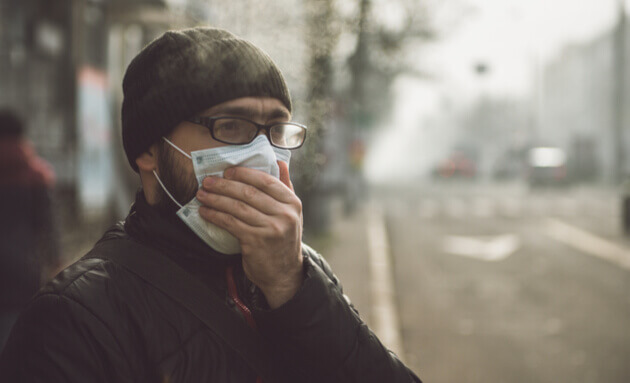
\includegraphics[width=\linewidth]{IMG/201912/image2}

\quad\quad Wearing masks under heavy air pollution is the most effective way of protecting ourselves, so choose proper masks and get the right fit becomes the next topic.

\quad\quad 在空气污染严重的情况下戴口罩是保护自己的最有效方法,因此,选择合适的口罩并正确佩戴将成为下一个课题。}

\subsection*{Know Your Mask Type 了解类型}

You can begin by \textit{evaluating(评估)} the levels of pollution in your area and accordingly opt for N-99, N-95 or N-100 masks. N-95 masks, as their name suggests will protect you from 95\% of all pollutants and fine particulate matter, while N-99 masks will offer you a higher level of protection and protect you from 99\% of all pollutants. You can also look for P-100 masks if you live in areas contain heavy oil-based pollutants.Look out for variants contain activated carbon filters as they can also help in absorbing bad odours, bacteria and viruses.



可以先评估你所在地区的污染水平,然后选择N-99,N-95或N-100口罩。 顾名思义,N-95口罩可保护你免受95%的所有污染物和细小颗粒物质的侵害,而N-99口罩将提供更高的防护水平——保护你免受99%的常见污染物的侵害。如果你居住在含重油基污染物的区域,也可以使用P-100口罩。注意含有活性炭过滤器的种类,因为它们也可以帮助吸附异味,细菌和病毒。
\begin{table}[H]
    \centering
    \caption{\kaishu 美国NIOSH标准对口罩的分类}
    \small
    \begin{tabular}{cccc}
    \toprule
     {\tiny 过滤效率} & $\ge$95\% & $\ge$99\% & $\ge$99.97\% \\
     \midrule
     N & N95 & N99 & N100\\
     R & R95 & R99 & R100\\
     P & P95 & P99 & P100\\
     \bottomrule
    \end{tabular}
    \label{tab:my_label}
\end{table}
\vskip-1em
{\small\kaishu

\noindent ·N:适合于过滤非油性颗粒物;

\noindent ·R:适合于过滤油性和非油性颗粒物;

\noindent ·P:适合于过滤油性和非油性颗粒物。

}
\subsection*{Fit Your Face 紧贴面部}

Ensure that your air mask \textit{seamlessly(无缝)} fits over your nose, mouth and chin. This is extremely \textit{vital(重要)} since a poor fit will allow harmful pollutants to seep into your mask thereby undoing all the good work put in by your mask.

确保口罩无缝贴合你的口鼻和下巴。 这至关重要,因为不合适的配戴会使有害的污染物渗入你的口罩,从而使口罩无法发挥最大作用。

\subsection*{Proper Storage 合理存放}

Masks designed for extended use must be cleaned and stored properly when not in use. Masks can themselves become infected with \textit{pathogens(病原体)}like bacteria and viruses, if not cleaned and aired properly. Improper storage might lead to breakage of the nose clip, while the \textit{elastic(弹性)}bands that secure the mask may lose their elasticity with extended use, causing an improper face-mask seal.

长期使用的口罩在不使用时必须清洁并妥善存放。 如果在没有经过合理清洁和通风的情况下,口罩本身可能会被细菌、病毒等病原体感染。存放不当甚至可能会导致鼻夹断裂;而固定口罩的松紧带可能会因长时间使用而失去其弹性,从而导致口罩密封不当。\EOA
\end{multicols}
\vskip-5em
\makeheading{课内知识拓展·酶促反应与催化剂原理}

\begin{multicols}{3}
酶促反应(\textit{又称酶催化})是指由一类被称为酶的特殊蛋白质所催化的化学反应。酶促反应的机制与其他类型的化学催化在原理上很相似。酶通过提供替代反应路线以及稳定中间产物的方法,减少了为达到最高能量过渡态时的能量需求。激活能($E_a$)的减少增加了具有足够达到激活能并形成产物的反应物分子的数量。


\begin{figure}[H]
    \centering
    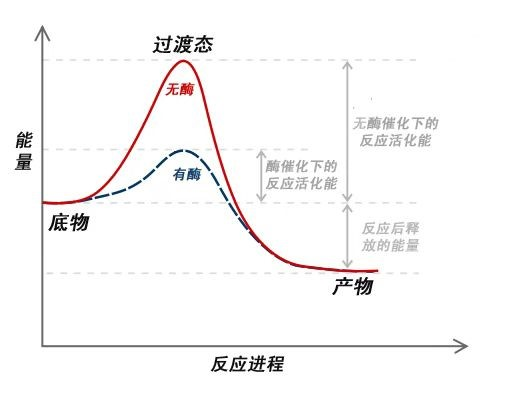
\includegraphics[width=\linewidth]{IMG/201912/23.jpg}
    \caption{\kaishu 酶使得中间状态达到稳定}
    \label{fig:my_label}
\end{figure}


最受欢迎的酶-底物反应模型是诱导契合模型。该模型提出了:酶和底物之间的最初反应是相对较弱的,但这些弱反应迅速引导酶中的构象改变以使结合变得更加紧密。

\begin{figure}[H]
    \centering
    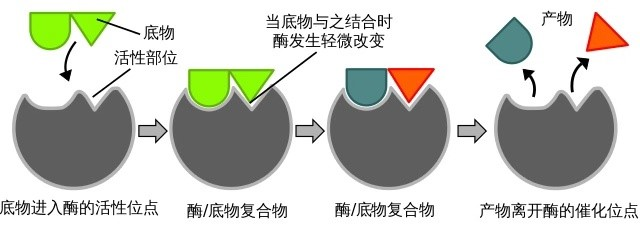
\includegraphics[width=\linewidth]{IMG/201912/123.jpg}
    \caption{\kaishu 酶反应诱导契合学说的图解}
    \label{fig:my_label}
\end{figure}


现在,我们由相对特殊的酶促反应过渡到全部催化反应的讨论中来。
催化剂的作用是改变反应路径,也就是改变基元反应(\textit{即最简单的化学反应步骤})。不同基元反应对应的活化能不同,从而通过这种办法提高了反应速率。

例如,双氧水分解,如果不加二氧化锰,则为\ce{2H2O2 = 2H2O + O2}↑

如果加上二氧化锰,则会先后发生下列两个基元反应:
\begin{center}\small
\ce{H2O2 + MnO2 = H2O + MnO + O2}↑

\ce{MnO + H2O2=H2O + MnO2}
\end{center}

由于反应(1)的活化能远远低于双氧水直接分解,所以体系中主要发生的是(1)(2)。这样双氧水生成氧气的速度就会大大提高。我们看到,二氧化锰在反应前后,总质量并没有改变,但它确实参与了反应。

因此,催化剂的定义是:参与反应,并能改变反应路径的媒介。催化剂的重要性质就是反应前后质量不变。\EOA

\end{multicols}
\ADxinhangdao

\newpage

\makeheading{生活中的科学·上期答案}

\begin{multicols}{3}
\noindent\qiangdiao{Q1 使用电脑的时候到底是要充着电用还是快没电了再充电?}

曾听说过这样一种说法,刚买回来的手机前几次使用要先充满电,再把电量耗尽,这样反复几次才能将电池激活,电池的寿命会更长。

如果说法是20年前的镍氢电池,这样做确实有一定科学道理。因为它有所谓的“记忆效应”——电池放久了之后镍极板上的晶体会变得粗大,影响和电解液的接触,导致容量下降 。进行几次完全充放电让晶粒细化,让容量部分恢复,这就是所谓“激活”。

而现在手机电脑已经用上了锂离子电池。锂离子电池是基于锂离子在插层化合物中嵌入脱出,并不存在着什么“记忆效应”。({\kaishu 详见本刊2019年10月号})

但锂离子电池的循环寿命只有500次左右,那么要怎样才能让锂离子电池寿命延长?

锂离子电池的循环寿命一般是定义为:锂离子电池进行深度充放电时,其容量能保持在80\%以上的循环次数。深度充放电容易破坏锂离子电池中的微观结构,使得容量降低;其次,锂离子电池的容量在80\%以下并不意味着电池报废,只会让它贴上“不耐用”的标签。

因此,延长锂离子电池的方法是减少对电池深度充放电(\textit{当然更要避免过度充电,过度放电}),也就是要对锂离子电池浅充浅放:没充满电就用,没放完电就充。

\noindent\qiangdiao{Q2 为什么黑笔和红笔的笔芯后面都有一小条黄色的东西?}

\noindent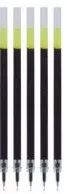
\includegraphics[angle=90,width=\linewidth,clip=true,trim=40 0 0 0]{IMG/201912/image11}
 
这段油状物就叫做随动密封剂,主要成分一般是锂基脂,它本身具有一定的粘稠度,而且也有很好的耐挥发性,主要的作用就是在笔管中油墨的末端保持良好的保湿密封,同时防止墨水倒流或者蒸发。

另外,随着笔芯的使用,笔管里的墨水量会逐渐减少。这时在外界大气压的作用下,锂基脂会往前移动,相当于往前“压油墨”以保证书写的顺畅——这时它相当于要起到“液体活塞”的作用。

\noindent\qiangdiao{Q3 为什么锯齿边可以帮助我们更容易撕开包装袋呢?}

\noindent
\includegraphics[width=\linewidth]{IMG/201912/image12.png}
   
在思考这个问题时我们可以建立一个简单的模型——当我们用同一种材料做成绳子时,如果做得中间细,两端粗,从两端拉绳子时,最容易断开是细的位置。因为沿绳子各处的张力是相等的,而细的地方承受能力更弱。我们可以进一步把包装的边缘想象成绳子(\textit{姑且称为“边缘绳子”}),而有缺口处就是比较细的位置(\textit{由于缺了一块,所以单位宽度承受了更大的拉力}),那么包装的边缘就更容易从缺口处裂开。当裂开以后,那么又形成了更大的缺口(\textit{“边缘绳子”的粗细之比就更大了}),从而更容易从缺口处裂开更大的缺口。于是,包装纸就容易撕开了。而这仅是一个比较简单的定性模型,实际操作过程中,“边缘绳子”的粗细比是很大的。因为我们通常不会拉住整个包装,而是只拉边缘的一点点,这就使得很结实的包装纸只要出现了缺口拉开都不是特别困难。
 


\noindent\qiangdiao{Q4 用盆接水,离水龙头近,接满水更快,还是离得远的快?}

在理想的条件下,考虑一个盆$A$在水龙头边上,另一个盆$B$在水龙头底下五米的距离,在0 s的时候开始出水(\textit{假设初始速度为}0 m/s),0 s时第一滴水以速度0 m/s的速度滴落到盆$A$,同等条件下,第一滴水需要走5 m,根据加速($g$=10 m/s$^2$)的计算,需要走1 s到达盆$B$,此时其速度为10 m/s. 假设60 s之后,盆$A$接满了水,拿走,总共用时60 s,61 s之后,盆$B$接满了水,拿走,总共用时60 s(61 s - 1 s),因此,无论是无论远近,水装满盆的时间一样. 

但是,在接热水时水龙头越高,水下降的速度越快,越容易喷溅,以及考虑到人需要先放盆再开水龙头的操作,推荐盆离水龙头更近些接水。\EOA

\end{multicols}
\vfil
\noindent\parbox{0.66\linewidth}{\greyboxNID{\vskip-43pt\makeheading{生活中的科学}\vskip1em

\quad\quad\parbox{0.9\linewidth}{\qiangdiao{Q1 为什么空杯子或者花瓶放到耳边会有声音?}

\rule{3ex}{0em}(Tips: 考虑管弦乐器的发声原理 )

\qiangdiao{Q2 为什么冷水冲不开咖啡?热水冲开之后不会沉淀?}

\rule{3ex}{0em}(Tips:考虑温度与溶解度之间的关系)

\qiangdiao{Q3 为什么自行车车胎充气后骑着轻,没气时重?}

\rule{3ex}{0em}(Tips: 考虑车胎机械能的转化与损耗)

\qiangdiao{Q4 为什么会形成白色的浪花?}

\rule{3ex}{0em}(Tips: 留意浪花中的气泡)}
\vskip1em}}\hfill
\parbox{0.3\linewidth}{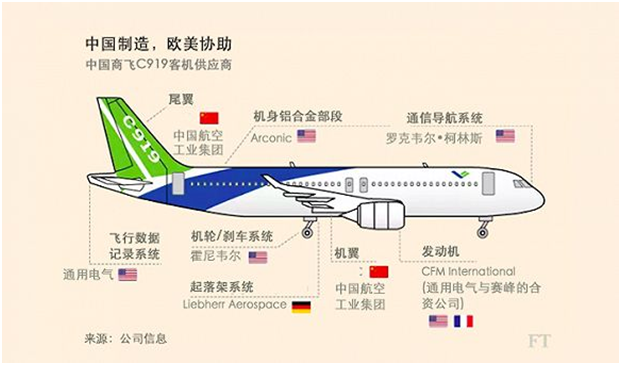
\includegraphics[clip=true,trim=40 0 40 0,width=\linewidth]{IMG/201912/20170511072434556.png}

\kaishu\quad\quad 国产大型客机C919的零件国产化率达到60\%,机身主体结构来自中航工业的各个公司,航电来自霍尼韦尔,发动机来自通用电气。\EOA}

\ADyixuehui



\newpage
\makeheading{港珠澳大桥岛隧工程的前世今生}

\begin{multicols}{3}
\greyboxNID{\kaishu

\quad\quad 港珠澳大桥连接香港、珠海、澳门,是世界最长的跨海大桥。该大桥部分以海底隧道代替桥梁,其主要原因是\uline{\qquad}(单选)。

\quad A.保障主航道通航能力 

\quad B.保障飞机起降安全

\quad C.避免气象灾害的影响

\quad D.减少泥沙淤积

}

这是2019级同学们当年地理中考的一道探究题,标准答案是单选A。由题目展开,我们来聊聊港珠澳大桥的核心控制性工程——这国际领先的岛隧工程。这两岛一隧,使港珠澳大桥备受国际桥梁工程界的瞩目。

\section*{桥隧之争}

港珠澳大桥横跨的珠江口水域是广州港、东莞港、中山港东部港区以及深圳港西部港区进出南海的\qiangdiao{唯一通道}。大桥依次跨越了九洲港航道、江海直达船航道、青州航道、榕树头航道、伶仃西航道和铜鼓航道西线。该水域通航密度大,年通航船舶达150万艘次。现在,一桥飞架粤港澳,水运通航如何保证?

国际上通行的答案是:航道桥。航道桥的净空高度高,且常用悬索来增大两桥墩间的距离,给船舶\qiangdiao{扩大通航空间}。大桥从西到东设置了九洲、江海、青州三座航道桥,净空高度从24.5米到42米,宽度173米到318米,\qiangdiao{与对应航道的通航船舶航行要求相适合。}其悬索主塔高都超过了一百米。

\begin{figure}[H]
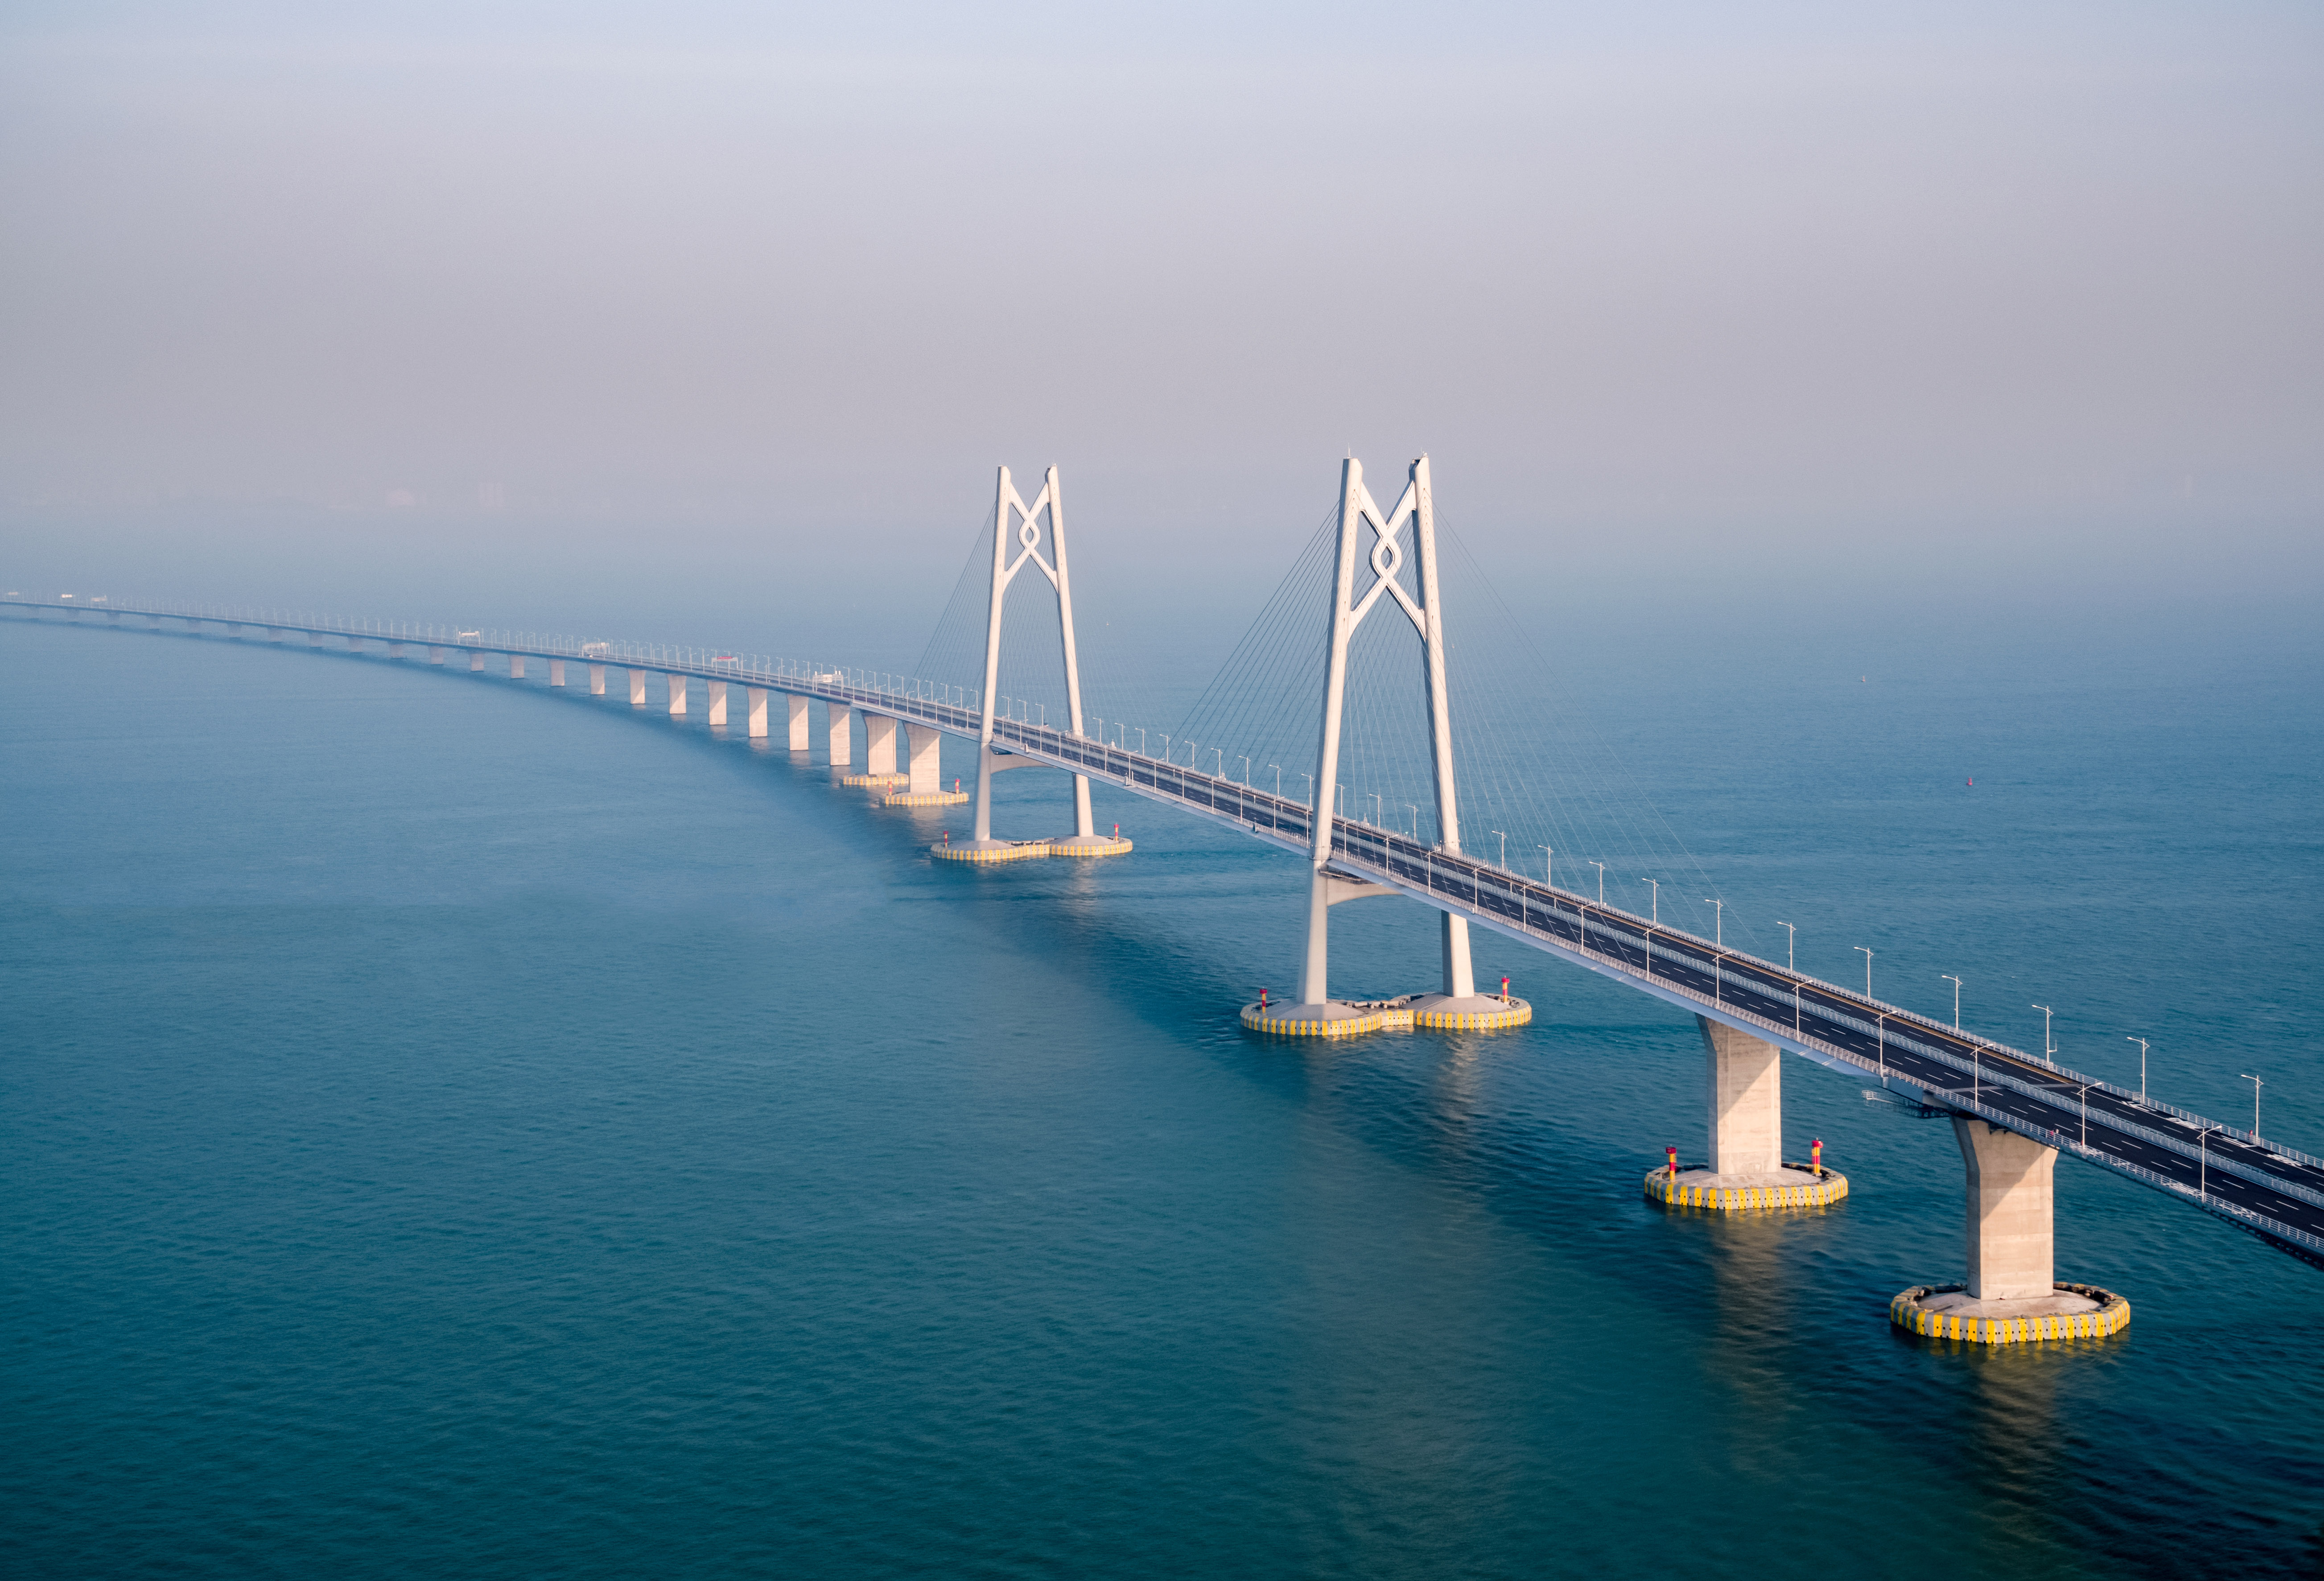
\includegraphics[width=\linewidth]{IMG/201912/Qingzhou-Bridge.jpg}
\caption{\kaishu 青州航道桥}
\end{figure}\vskip-1em

继续向东,来到珠江口最繁忙的伶仃西航道,这是进出世界第五大港广州港的\qiangdiao{十万吨级}巨轮航行的咽喉\ ,\\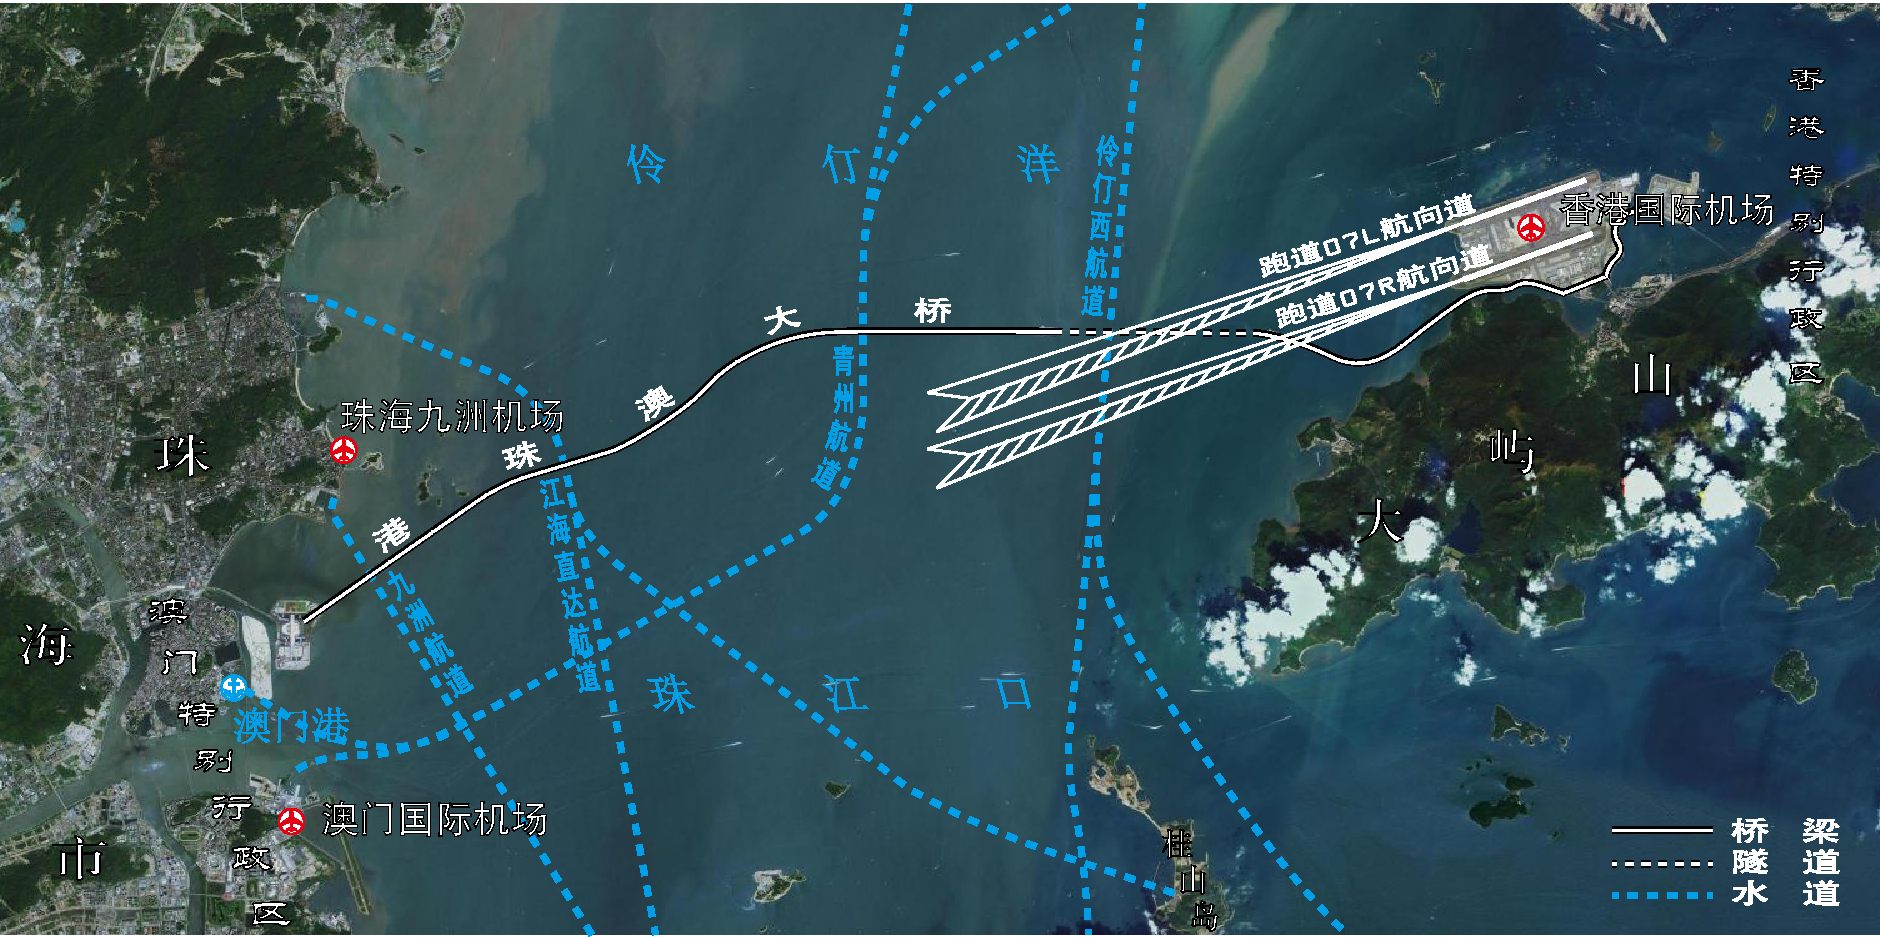
\includegraphics[width=2.13\linewidth]{IMG/201912/Map.pdf}%

\noindent 设计净空达到76.5米,如果按上述桥梁标准建设,主塔高可能会达到二百米。这座“没有建”的桥不光施工难度大,还会影响一个你想不到的地方——香港赤蠟角国际机场。

香港赤蠟角国际机场近年来成为\qiangdiao{世界货邮吞吐量第一、旅客吞吐量第八}的大型国际机场。1998年通航,目前建有两条远距平行跑道,规划有第三条平行跑道。

受制于盛行风、地形、管制区等因素,香港机场跑道的磁方位为73.9°/253.9°,呈东北西南走向。由于香港盛行东风,所以飞行器主用\texttt{07L/07R}跑道向东北起降。飞机降落时,会在跑道延长线上距跑道头约20km处转向对正跑道并下降高度。而跑道延长线与大桥最近交于6.5km,我们参阅香港民航处发布的公开进近航图,可以得知飞机在此处的高度约为295m。

如果按照之前计算的航道桥建设,那么桥梁主塔将与进近的飞机\qiangdiao{垂直距离过近},难以保证安全。飞机进近时下滑道低一点点,就有与桥塔相撞的危险。所以,港珠澳大桥在这一段,采用了沉管海底隧道的方案。

从长远来看,这一设计是明智的。哲学课本告诉我们:联系是普遍存在的,要用联系的观点看问题。广州港及周边港口年吞吐量巨大,未来极有可能通航更大吨级和高度的船只,如果因为这座大桥限制了港口之后的扩容,那未免就有些可惜了。



\rule{0em}{17.23em}

\section*{人工岛}

\begin{figure}[H]
    \centering
    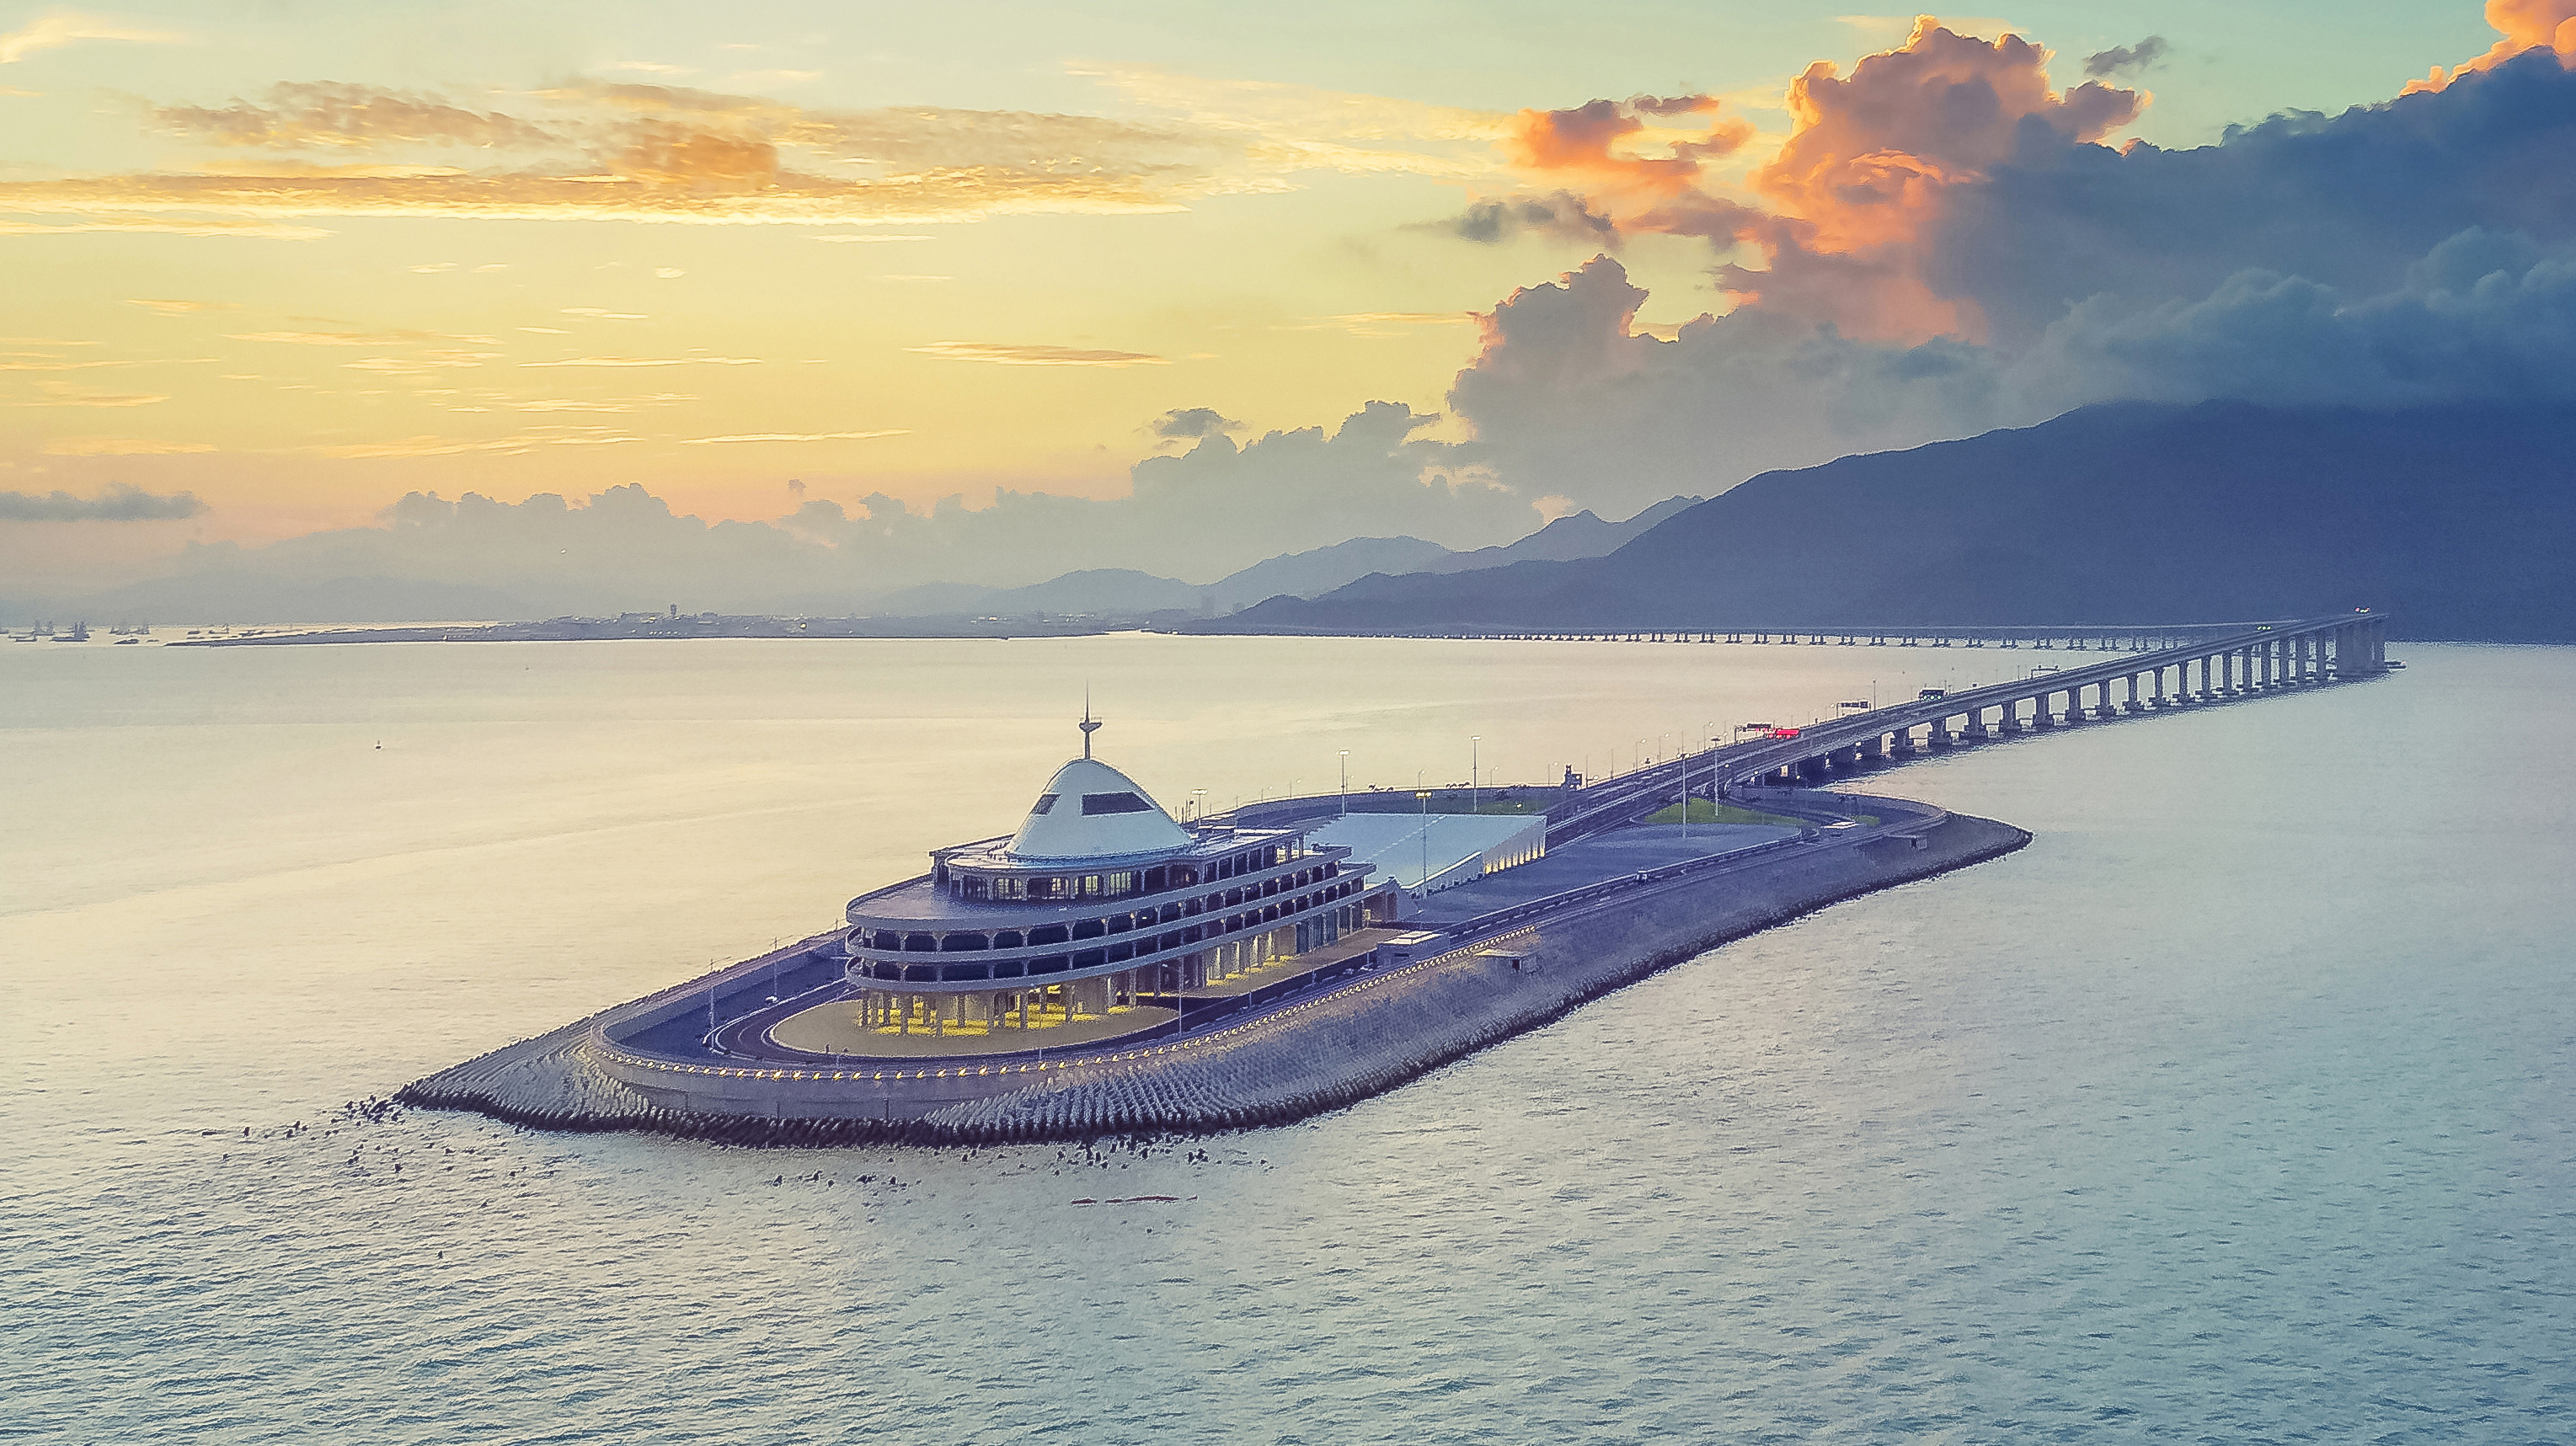
\includegraphics[width=\linewidth]{IMG/201912/East-Island.jpg}
    \caption{\kaishu 东人工岛}
    \label{fig:my_label}
\end{figure}

东西两个桥隧转换使用的人工岛,隔海相望,是整座大桥的看点。它们是填海造岛形成的,每个面积约为十万平方米,建设过程约7个月。其中,填海的过程非常复杂:


\qiangdiao{第一步:人工围堰。}将约61个直径 22 米,高 40 多米,重 500 吨的钢圆筒,利用 8 台振动锤直接插入软土层,到达海底坚固的不透水层后,再往圆筒内注入沙子,形成一个封闭海堤,再把内部的水抽干。

\qiangdiao{第二步:岛身填筑。}也就是往围堰里填沙子。西人工岛用的是平均直径 0.35mm 以上的中粗砂,从陆地通过船只运输而来。然后往沙土中打入外壁带孔的排水管道,利用沙土的重力挤压让水分渗到管道中再抽到岛外,使沙土紧实固结,这需要持续 4至5 个月。

\qiangdiao{第三步:修建护岸。}在钢圆筒外侧先挖掉淤泥后填入 2 米厚的碎石层,接着要靠砂桩船进一步加固土层。最后再抛入碎石堆成斜坡,放入扭工字块,形成护岸防止海浪侵蚀人工岛。这样,一座人工岛就建成了。

\section*{沉管隧道}

\begin{figure}[H]
    \centering
    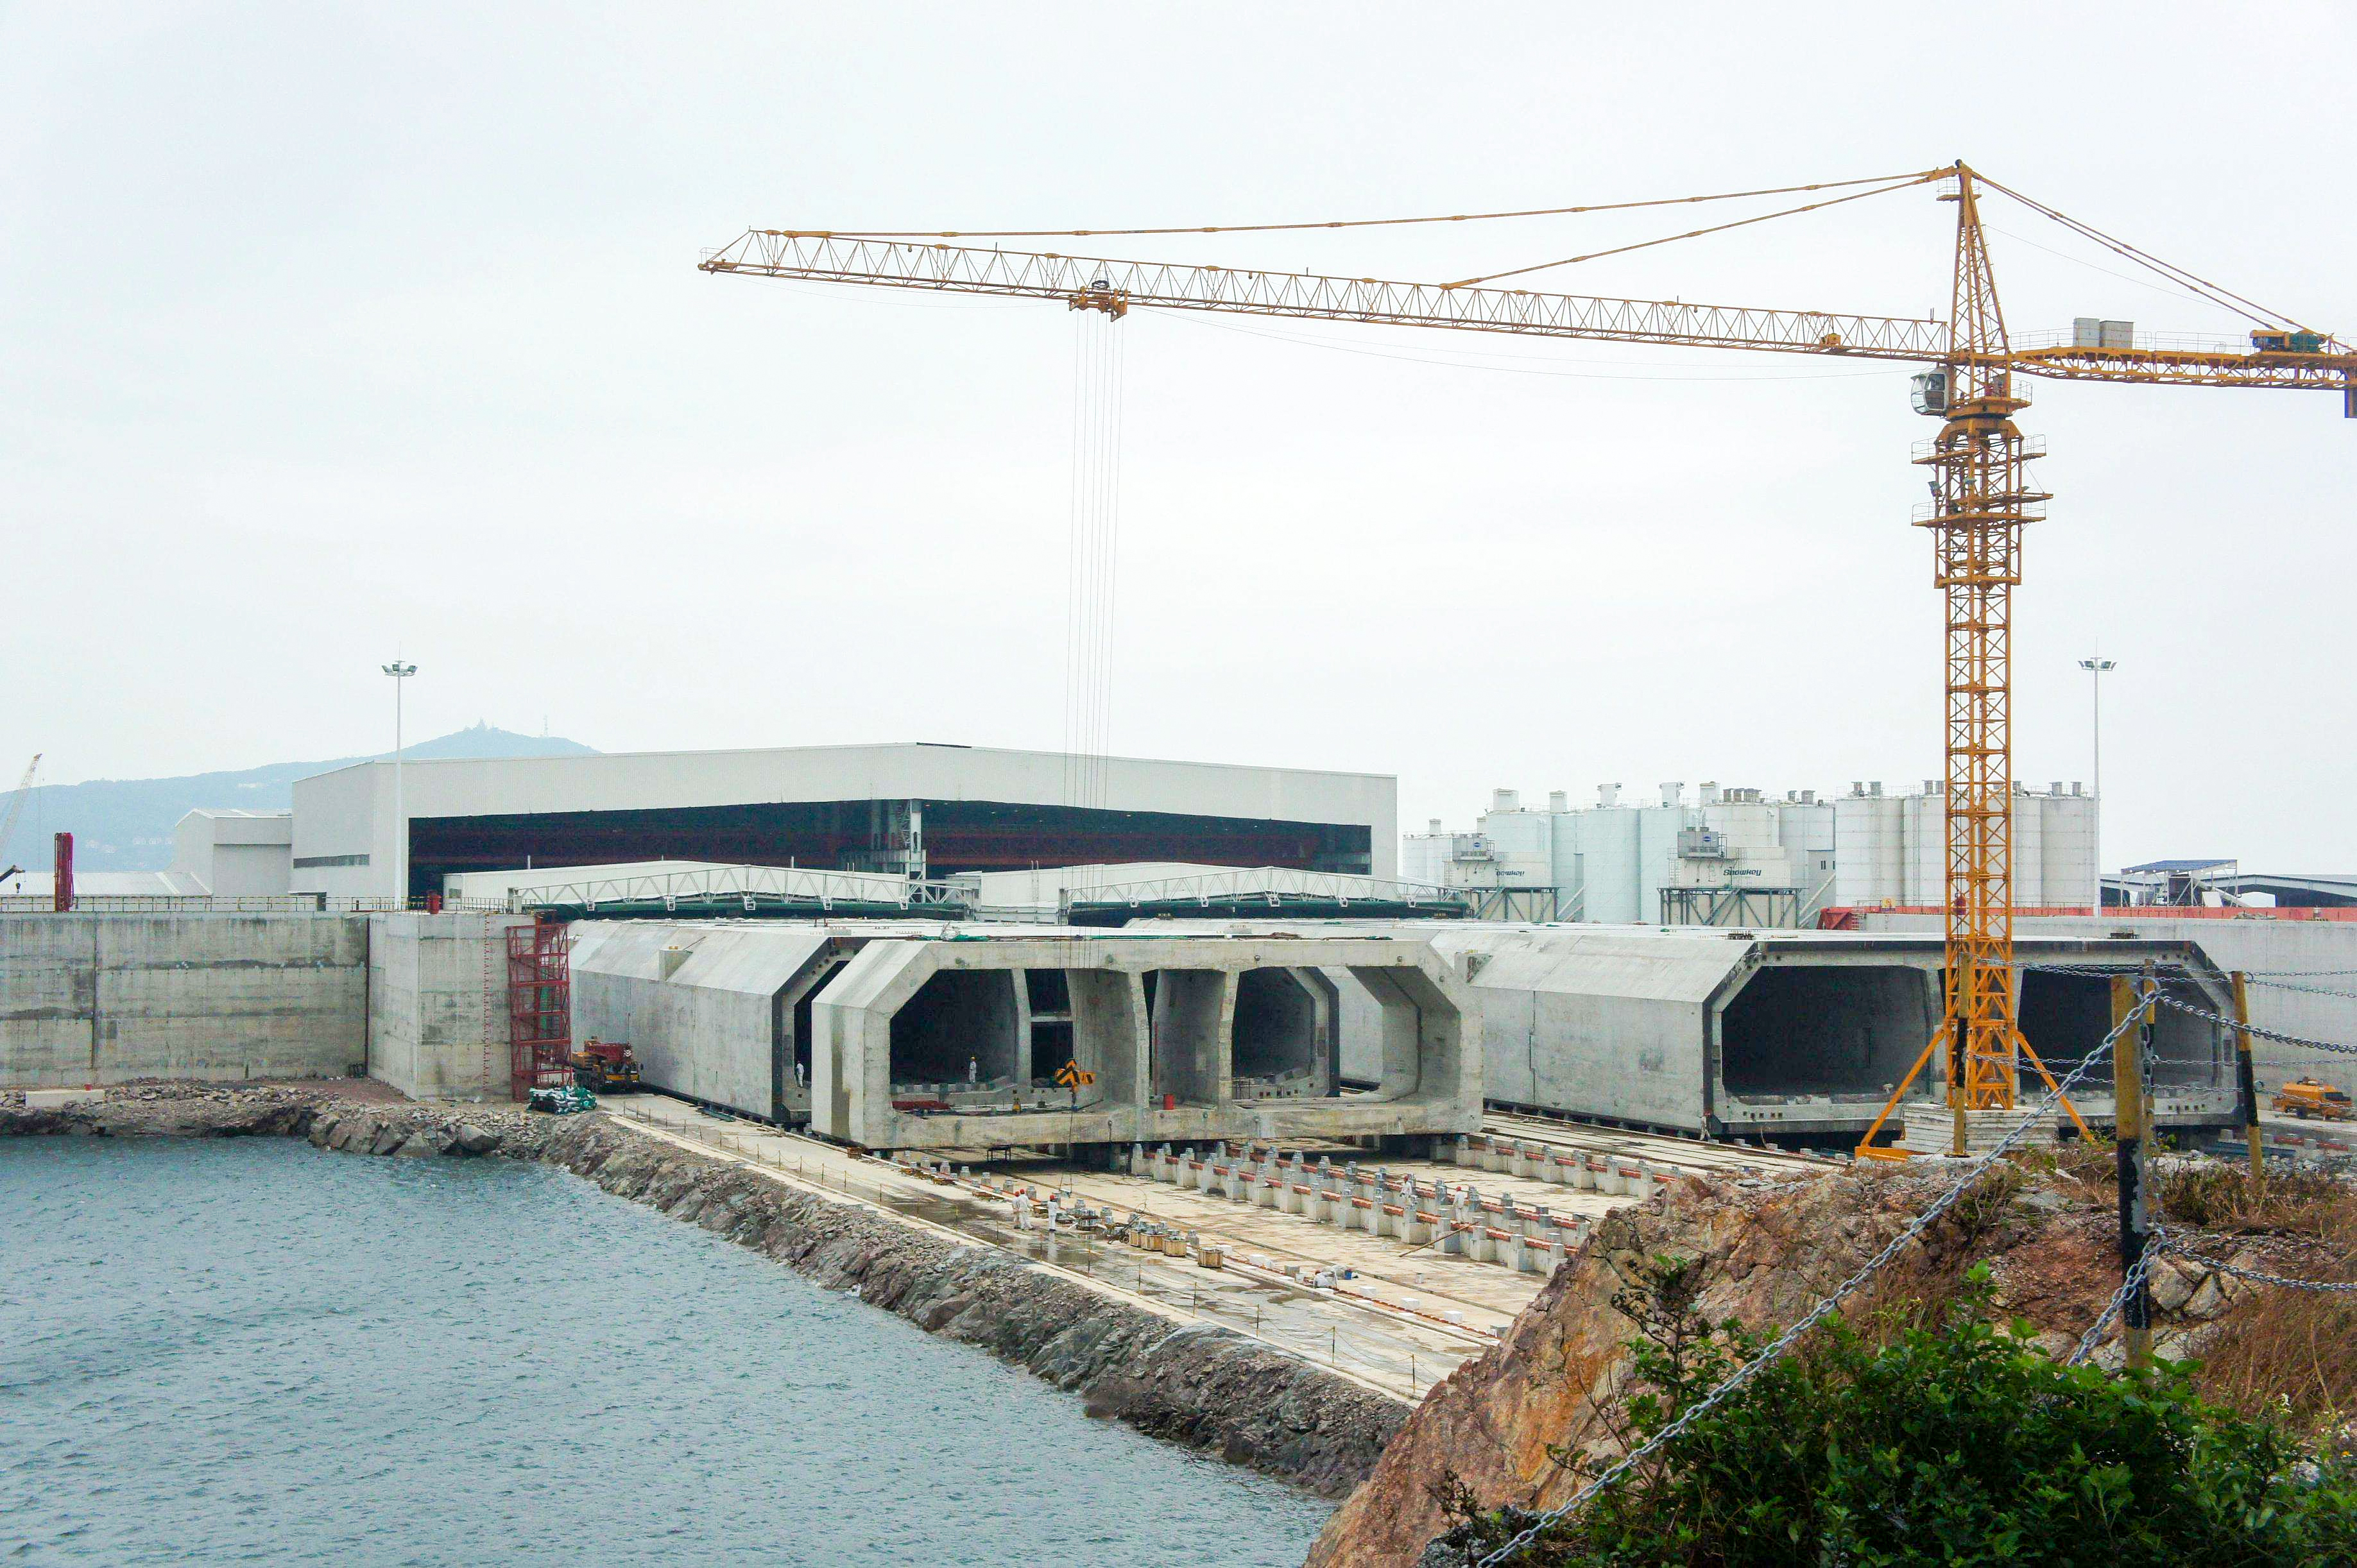
\includegraphics[width=\linewidth]{IMG/201912/Tube.jpg}
    \caption{\kaishu 等待入水的沉管}
    \label{fig:my_label}
\end{figure}

港珠澳大桥海底隧道是\qiangdiao{世界最长的公路沉管隧道和唯一的深埋沉管隧道},海底部分约5664米,由33节巨型沉管和1个合龙段最终接头组成,最大安装水深超过40米。

沉管工厂厂址选在施工现场以南约13公里的桂山岛上,东边就是大屿海峡的深水航道,便于沉管的运输。每节长沉管长180 米、宽38米、高11.5米,重达8万吨,堪比航母。

沉管用混凝土浇筑,完成后,由8台大马力拖船拖至安装地点。沉管下沉至准备好的海底基槽中,按相关参数要求进行精确定位,然后和前面已经安放好的管节进行对接。对接完毕后,在管节接头部位排水并浇筑混凝土,最后在沉管两侧和顶部进行砂石方回填和防护,一节沉管便安放完毕。

\section*{写在最后}
港珠澳大桥被誉为“新世界七大奇迹之一”,它的建设创下了多项世界之最。十年漫漫建设之路里,是几千名中国工程师逢山开路,遇水架桥的奋斗精神。一桥连三地,天堑变通途,这是中国力量,更是中华民族在“一国两制”框架下实现的一个伟大胜利。

回到题目,我个人认为,修建海底隧道的主要原因是机场的净空限制,根本原因才是保证主航道通航。出题老师既然出了B项,图中也标注了香港机场,说明他很可能是知道这个原因的。其实C、D项也有道理,但答案是单选A或许只是想让大家得分不那么困难吧。

推荐大家阅读何建明的纪实著作《大桥》,它以岛隧工程总设计师林鸣为主人公,用非虚构的手法描绘了工程建设的细节,值得一读。\EOA

\end{multicols}
\vskip-5em
\makeheading{科技快讯}
\begin{multicols}{3}
\subsection*{LIGO引力波望远镜观测能力升级}

\noindent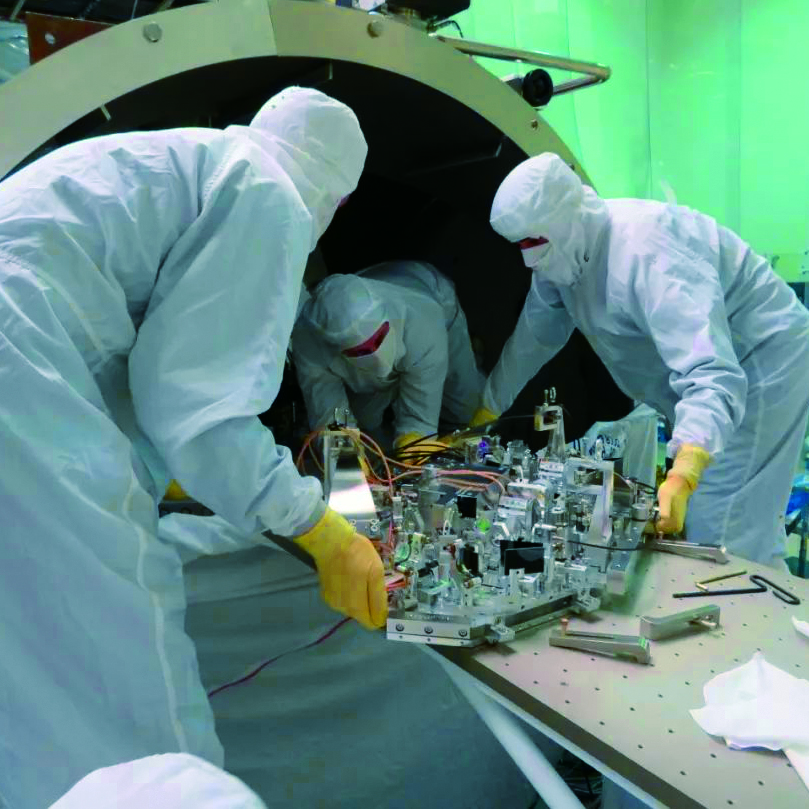
\includegraphics[width=\linewidth]{IMG/201912/111.jpg}

最近,LIGO望远镜增添了用于探测引力波的新仪器——量子真空挤压机。该仪器使得研究人员几乎每周都能观测到引力波,因为它可以减少量子噪音背景,即一些真空中的波动对观测结果的影响。虽然这些噪音背景本身十分微弱,但在观测时它会与望远镜所用的激光中的光子互相干扰,对引力波信号的测量造成影响。在新仪器的帮助下,LIGO望远镜的探测距离增加了15\%,可观测到4亿光年外产生的引力波信号。

\subsection*{北斗三号全球核心星座部署完成}

\noindent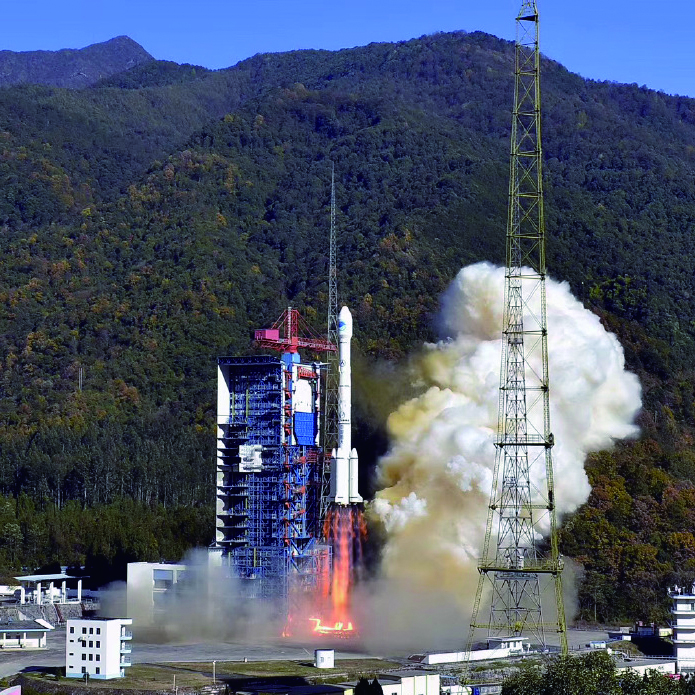
\includegraphics[width=\linewidth]{IMG/201912/1112.jpg}

2019年12月16日15时22分,我国在西昌卫星发射中心用长征三号乙运载火箭及远征一号上面级,以“一箭双星”方式成功发射第52、53颗北斗导航卫星。至此,所有中圆地球轨道北斗卫星全部发射完毕,标志着北斗三号全球系统核心星座部署完成,以平均每月1.2颗的高密度,刷新全球卫星导航组网速度世界纪录。这将进一步提升北斗卫星导航系统的服务性能和用户体验,为实现全球组网奠定坚实基础。

\subsection*{首颗被确认进入太阳系的系外彗星}

\noindent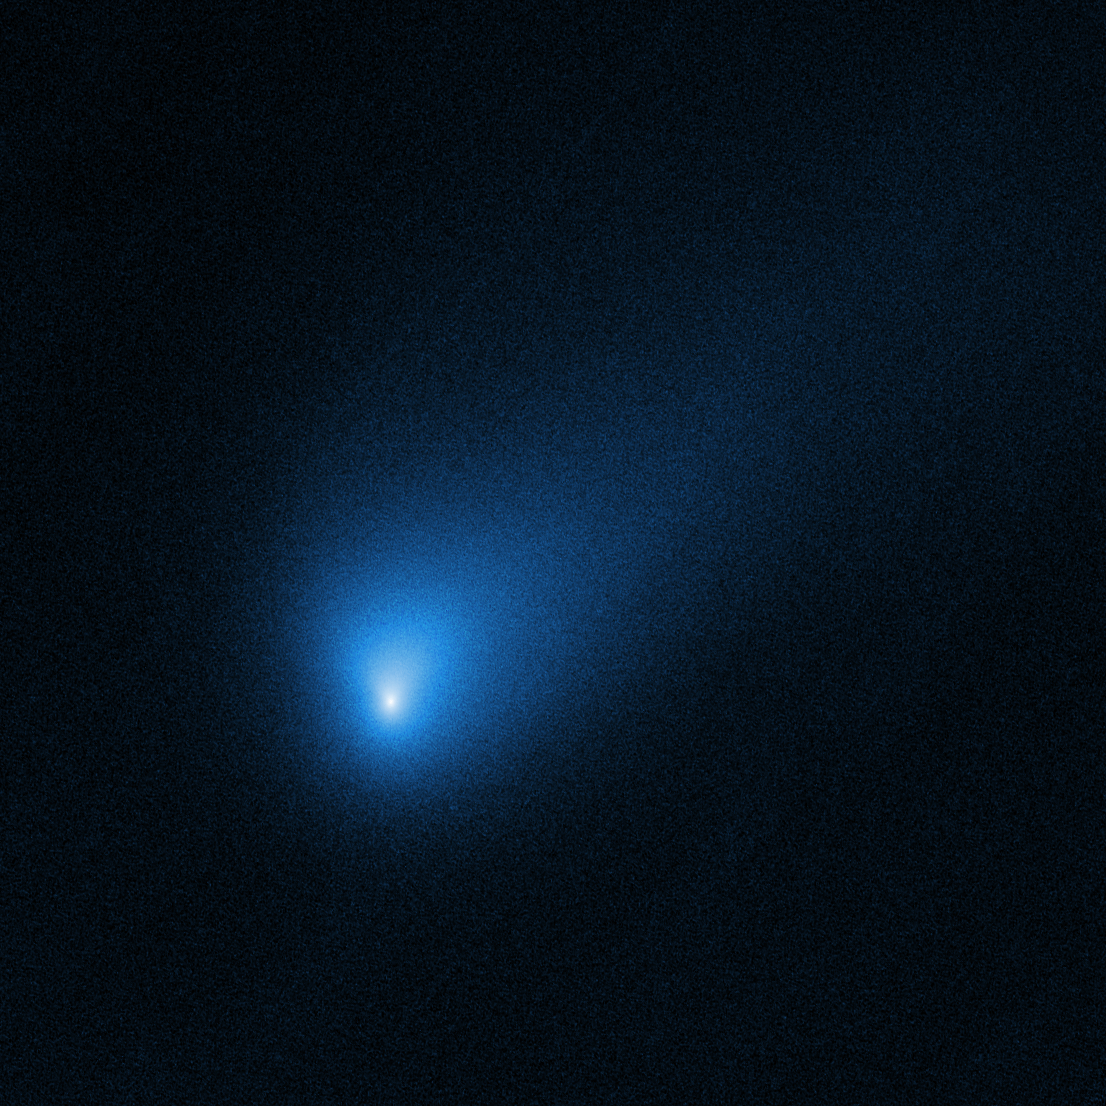
\includegraphics[width=\linewidth]{IMG/201912/stsci-h-p1953a-f-1106x1106.png}

NASA称哈勃太空望远镜拍摄到了代号为2I/Borisov的彗星的新图像,这是首颗被确认从星际空间进入太阳系的彗星。这是天文学家发现的首颗系外彗星。哈勃望远镜的图像捕捉到了该彗星在我们的太阳系中飞奔,并将在2020年中返回星际空间。许多望远镜的观测表明,这颗彗星的化学成分类似于我们自己太阳系中发现的彗星,这证明明彗星也能在其他恒星周围形成,并被弹出到宇宙深空。\EOA
\end{multicols}

\ADhairui



